\section{支架三维建模分析}

\subsection{切割法建模}
所谓切割法是从具备包容待建模模型基本形体之中逐步切除多余部分,从而实现三维模型构构建的方法。图\ref{fig:zhijiafenxi0}为构建支架模型的基本楔体,在此基础之上去除圆角之外多余部分材料构成图\ref{fig:zhijiafenxi1}的结果,图\ref{fig:zhijiafenxi2}是去除孔材料的结果,图\ref{fig:zhijiafenxi3}是去除中间部分多余材料的结果。其整个过程是不断的切除多余的材料来实现支架模型。

\begin{figure}[htbp]
\centering
\subfloat[]{\label{fig:zhijiafenxi0}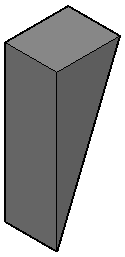
\includegraphics[scale=0.5]{zhijiafenxi0}}\hspace{20pt}
\subfloat[]{\label{fig:zhijiafenxi1}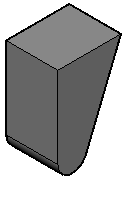
\includegraphics[scale=0.5]{zhijiafenxi1}}\hspace{20pt}
\subfloat[]{\label{fig:zhijiafenxi2}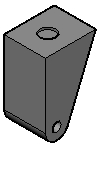
\includegraphics[scale=0.6]{zhijiafenxi2}}\hspace{20pt}
\subfloat[]{\label{fig:zhijiafenxi3}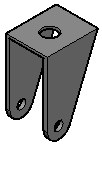
\includegraphics[scale=0.6]{zhijiafenxi3}}
\caption{切割法建模支架}
\end{figure}

\subsection{叠加法建模}

所谓叠加法是将待建模的形体切割为多个组成部分,然后将各个组成部分叠加组合在一起来构建三维模型的建模方法。图\ref{fig:zhijiafenxi4}的平板和图\ref{fig:zhijiafenxi5}的支耳是支架的基本组成部分,将两部分有效的组合在一起即可构建图\ref{fig:zhijiafenxi6}所示的支架三维模型。

\begin{figure}[htbp]
\centering
\subfloat[]{\label{fig:zhijiafenxi4}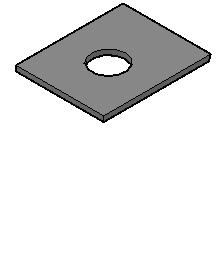
\includegraphics[scale=0.5]{zhijiafenxi4}}\hspace{20pt}
\subfloat[]{\label{fig:zhijiafenxi5}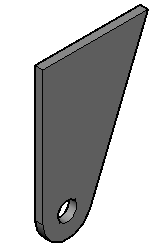
\includegraphics[scale=0.5]{zhijiafenxi5}}\hspace{20pt}
\subfloat[]{\label{fig:zhijiafenxi6}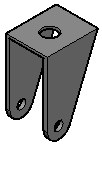
\includegraphics[scale=0.9]{zhijiafenxi3}}
\caption{叠加法建模支架}
\end{figure}

在实际的模型构建过程中经常需要将叠加建模法和切割建模法组合起来运用,如图\ref{fig:zhijiafenxi4}的平板和图\ref{fig:zhijiafenxi5}的支耳中的孔是运用切割法来完成。

\endinput